%In this section we provide details of the three datasets that we evaluate in this paper, as well as the methodology used.
%\subsection{Dataset description}


%\subsubsection{Twitter example (Detection of natural disasters)}
We now describe the dataset and baselines used in our experiments.

\subsection{Dataset description}
The scenario we have chosen to evaluate our algorithms is related to the detection of natural disasters discussed in a collection of tweets chosen due to the availability of high volume spatio-temporal data and it's general familiarity to our human test subjects.  
We started with a corpus of approximately 1 billion tweets crawled from the Twitter streaming API during 2013 and 2014 with the following restrictions:
%the Twitter data described in~\cite{Iman2017}:
%, which was curated by four students as follows: 
(1) the dataset was restricted to users located within the US, (2) non-English tweets were filtered out, (3) we extracted tweets related to the 12 actual natural disasters 
 described in Table~\ref{tbl:events}
%(a storm, a hurricane,  a drought, two floods, two earthquakes, two tornadoes,  and three blizzards) 
-- which are temporally and geographically disjoint -- to use as ground truth clusters, and (4) we removed tweets related to other known natural disasters to create unambiguous correct answers. 
% for use in our human subject experiments. 

%a storm, a hurricane,  a drought, two floods, two earthquakes, two tornadoes,  and three blizzards. 
%and finally, (4) false positive tweets (i.e., tweets mentioning natural disaster specific-keywords but not related to a particular natural disaster) from the dataset were intentionally included, e.g., \textit{\textquotedblleft I'm flooded with questions from followers\textquotedblright{}}. The final dataset contains 39,486 tweets with 5,075 marked as relevant tweets.% (a relevant tweet is a tweet related to a natural disaster).

% Preview source code for paragraph 0

\begin{table}[t]

\caption{Details of the events included in the dataset.}
\label{tbl:events}
\begin{centering}
\begin{tabular}{|c|c|c|c|c|}
\hline 
 & \textbf{Type} & \textbf{Location} & \textbf{Date} & \textbf{\#tweets}\tabularnewline
\hline 
\hline 
1 & Tornado & Mississippi & Feb, 2013 & 564\tabularnewline
\hline 
2 & Tornado & Oklahoma & May, 2013 & 893\tabularnewline
\hline 
3 & Storm & Florida & June, 2013 & 564\tabularnewline
\hline 
4 & Flood & Colorado & Sep, 2013 & 201\tabularnewline
\hline 
5 & Drought & CA & Dec, 2013 & 258\tabularnewline
\hline 
6 & Blizzard & NY & Feb, 2014 & 249 \tabularnewline
\hline 
7 & Earthquake & LA, CA & Mar, 2014 & 344\tabularnewline
\hline 
8 & Blizzard & Boston, MA & June, 2014 & 412\tabularnewline
\hline 
9 & Hurricane  & North Caro. & July, 2014 & 420\tabularnewline
\hline 
10 & Earthquake & Nappa, CA & Aug, 2014 & 416\tabularnewline
\hline 
11 & Flood & Michigan & Aug, 2014 & 528\tabularnewline
\hline 
12 & Blizzard & Buffalo, NY & Nov, 2014 & 249\tabularnewline
\hline 
\end{tabular}
\par\end{centering}
\end{table}



\subsection{Baselines description}
Experiments use the following two baseline clustering algorithms:

\subfour{Optimal solution:} To benchmark the performance of {\bf Greedy} and {\bf BPS} on small datasets, we use an exact Mixed Integer Linear Progamming (MILP) optimization-based formulation to maximize EF1. In brief, the formulation of EF1 in~\eqref{eq:EF1} can be transformed into a \emph{fractional} MILP formulation with constraints corresponding to each of the cluster attribute selection criteria (space, time, and content). The parameters of these constraints are then chosen to optimize the EF1 objective.  While there are no direct solvers for fractional MILPs, we can transform the problem into a pure MILP formulation using the Charnes-Cooper method \cite{Charnes1962} and Glover linearization method \cite{Glover1975} for which we have optimal (albeit slow) solvers .% with big-M constraints.  
%Lastly, we add three constraints to the optimization to select elements through three clustering parameters, i.e., time, position and keywords. %We refer the reader to [ADD ANONYMOUS CITATION?] for more details o this method.




 
\subfour{$K$-means clustering:} We use the $X$-means~\cite{Pelleg2000} variant of $K$-means as a baseline method to {\bf cluster matching search results}. $X$-means is a simple extension of $K$-means~\cite{kmeans_original} that tries to  automatically determine the number of clusters. Starting with only one cluster, the $X$-means wrapper applies after each run of $K$-means, making local decisions about which subset of the current centroids should split themselves in order to better fit the data.  In order to provide $X$-means with spatial, temporal, and content coherence, the distance metric we have used for $X$-means is a linear combination of the following: (i) the Euclidean distance of time, (ii) the Euclidean distance of location, and (iii) the cosine distance of the textual content. This distance metric is formally defined as follows:
%\begin{equation}
%\begin{array}{ll}
%d(i,j)= & \alpha\times\textrm{[time distance]} +\\
%& \beta\times\textrm{[location distance]}+\\
% & \gamma\times\textrm{[text cosine distance]}
%\end{array}
%\end{equation}
\begin{equation}
d(i,j)=  \alpha\times\textrm{[time dist.]} +
 \beta\times\textrm{[location dist.]}+
  \gamma\times\textrm{[text cosine]}
\end{equation}
where $\alpha$, $\beta$, and $\gamma$ are weights that sum to 1, %set all to 1 in the off-line evaluation 
and set respectively to 0.1, 0.8, and 0.1 in the user study -- values tuned by grid search to maximize sum of EF1 scores given data from Table~\ref{tbl:events}.  Once clusters are extracted by $X$-means, we use the EF1 metric to extract the top clusters as required by our interface.

%We assume having an agent monitoring tweets, a topical tweets classifier (e.g., \cite{Iman2017}), and a display showing the locations of the tweets (See Figure \ref{Fig:TwitterData}).  We used the  2.5 TB of Twitter data described in  \cite{Iman2017}, for which we restricted our analysis to the 9M tweets of January 2014.





%\begin{figure}[t]
%\begin{centering}
%\subfigure[Twitter Networks.]{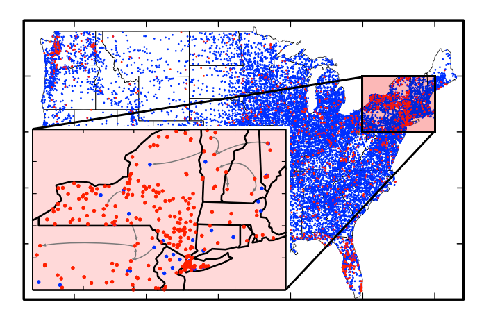
\includegraphics[width=2.8cm]{imgs/twitter_example_3}\label{Fig:TwitterData}}\subfigure[Enron Networks.]{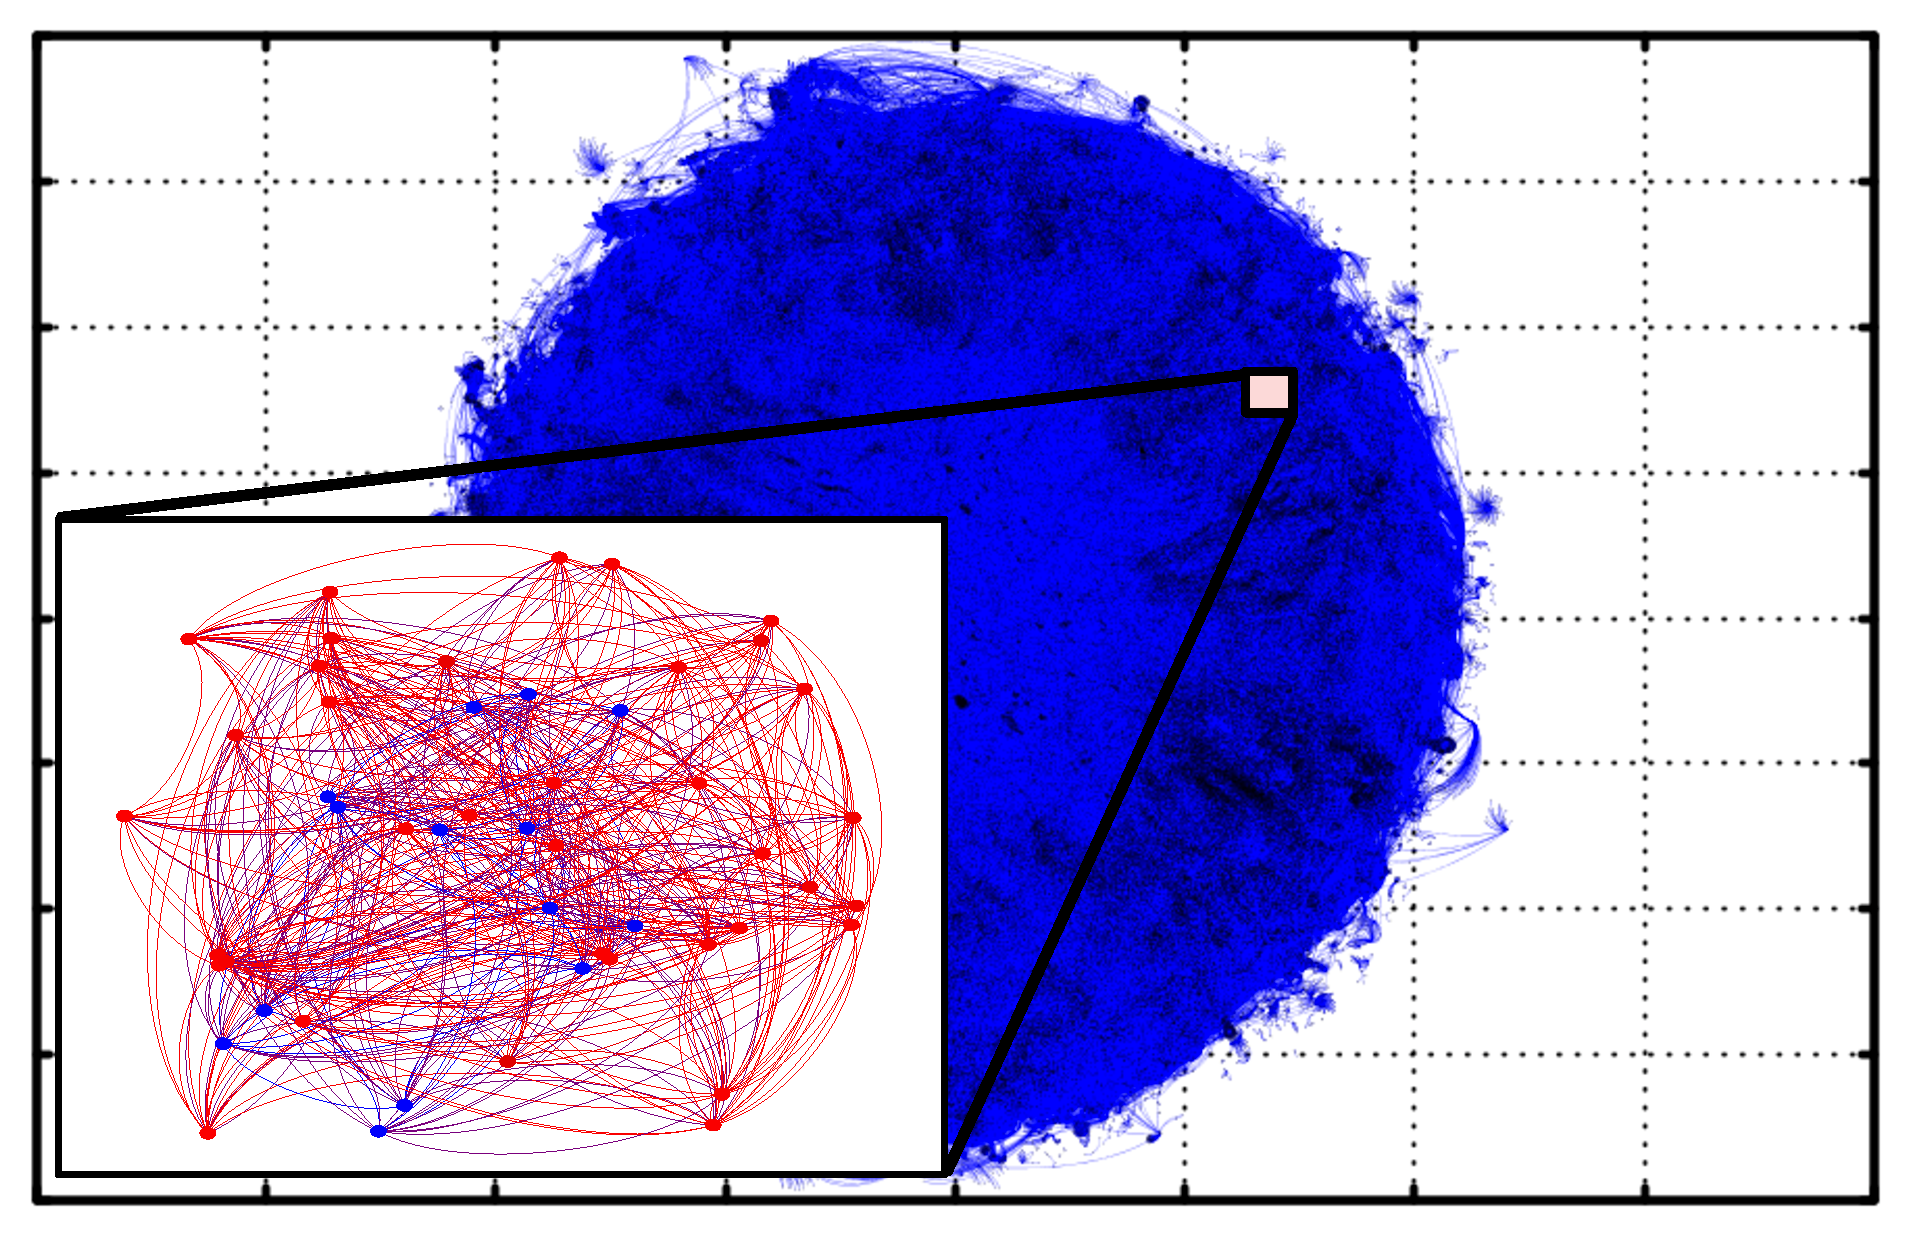
\includegraphics[width=2.8cm]{imgs/enron_net_4}\label{Fig:EnronData}}\subfigure[Reddit Networks.]{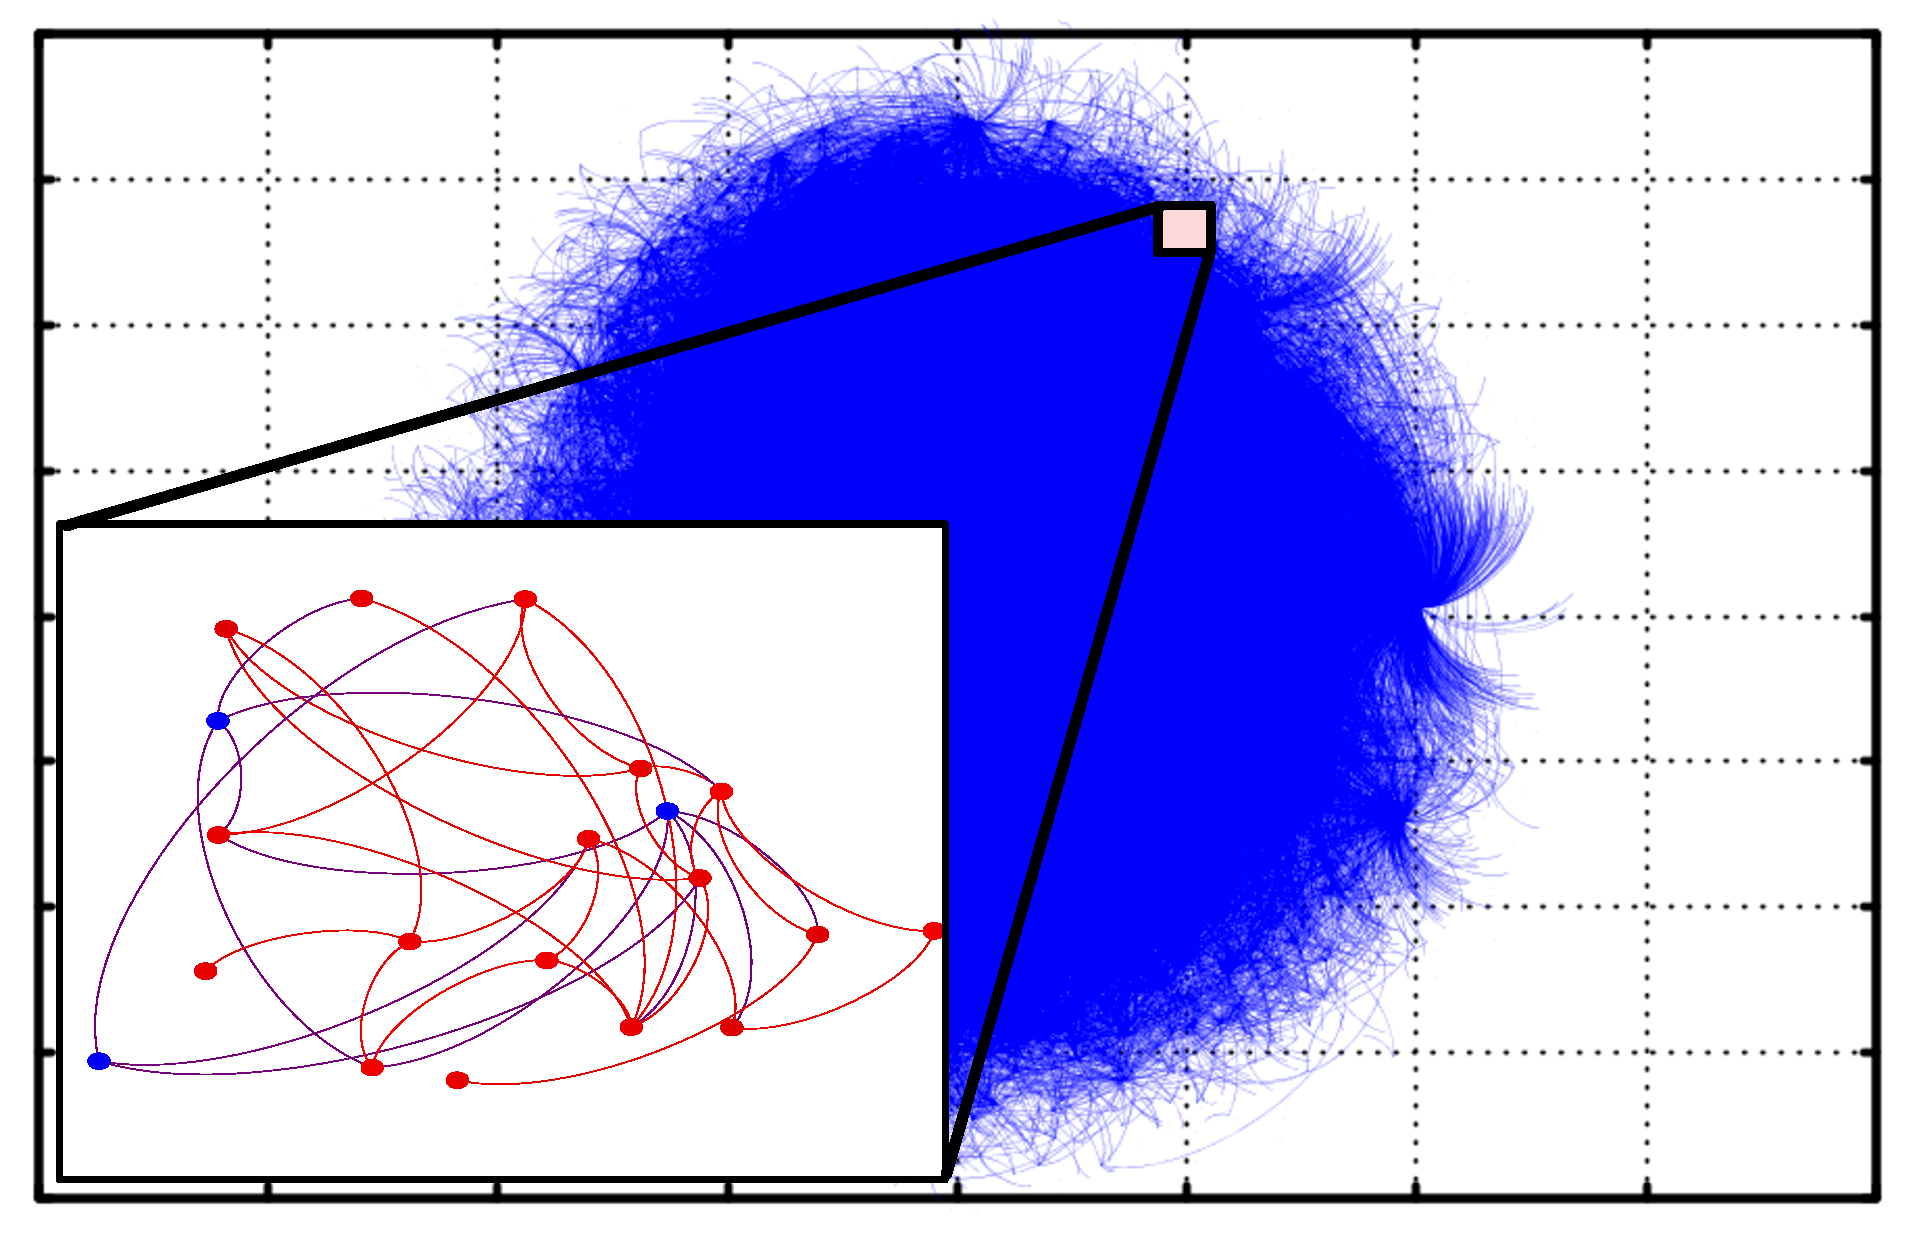
\includegraphics[width=2.8cm]{imgs/srforum3}\label{Fig:RedditData}}
%\par\end{centering}
%\caption{Layouts used for the different datasets.}
%\end{figure}





